\chapter{Diagramas}

\section{Diagrama de componentes}

En este diagrama se visualiza la arquitectura de componentes de la plataforma, mostrando la interacción entre la interfaz web, los módulos encargados del procesamiento de las métricas y los componentes responsables de la detección y análisis de anomalías. Se representa el recorrido de la información desde la infraestructura de Huawei Cloud y el usuario, pasando por la API de backend, la recolección y transformación de los datos, el modelo de Isolation Forest y el motor de recomendaciones, hasta el almacenamiento de los resultados en PostgreSQL y su posterior utilización para la generación de reportes y visualización.

\begin{figure}[htbp]
\centering
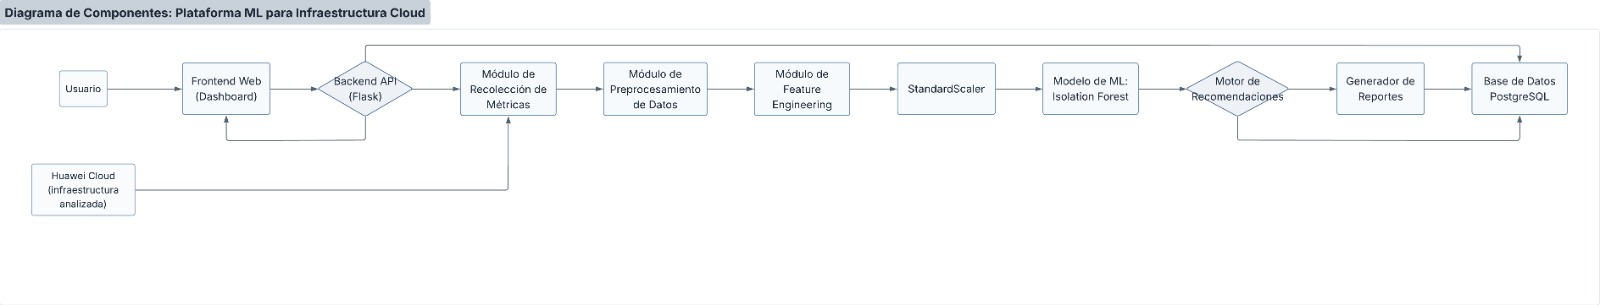
\includegraphics[width=0.9\textwidth]{media/image3.png}
\caption{Diagrama de componentes de la plataforma}
\label{fig:componentes}
\end{figure}

\section{Diagrama de flujo}

El siguiente diagrama presenta el flujo general de información de la plataforma, desde la obtención de las métricas de la infraestructura cloud hasta la generación y visualización de los resultados. Se detallan las principales etapas de procesamiento, incluyendo el preprocesamiento, la generación de características, la normalización y la detección de anomalías mediante Isolation Forest, seguida por el motor de recomendaciones cuando se identifica una instancia anómala. De esta manera, el diagrama permite visualizar de forma integral el recorrido de los datos dentro de la solución.

\begin{figure}[htbp]
\centering
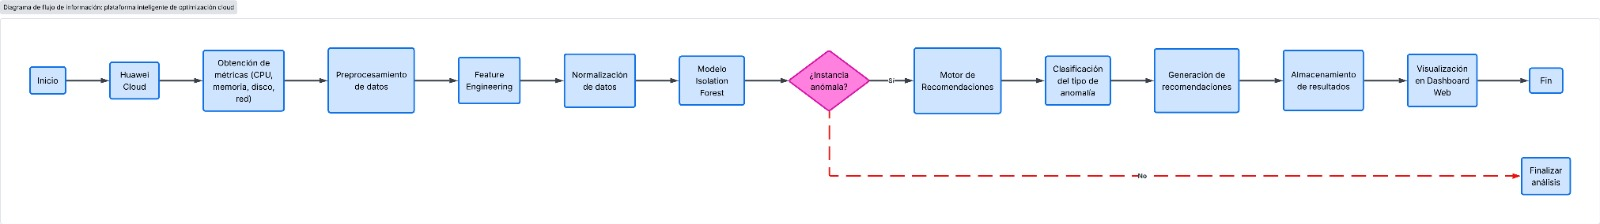
\includegraphics[width=0.9\textwidth]{media/image5.png}
\caption{Diagrama de flujo de la plataforma}
\label{fig:flujo}
\end{figure}

\section{Diagrama de arquitectura}

El diagrama de arquitectura presenta una visión general de la estructura tecnológica de la solución, mostrando la organización de los diferentes componentes y servicios que conforman la plataforma. Se observa la separación entre el frontend desarrollado con tecnologías web estándar, el backend implementado en Flask que actúa como intermediario entre la interfaz y los módulos de procesamiento, y los componentes especializados encargados de la comunicación con Huawei Cloud, la detección de anomalías mediante Isolation Forest y la generación de recomendaciones de optimización. Esta arquitectura modular permite que cada componente cumpla una función específica, facilitando la mantenibilidad del sistema y la incorporación de nuevas funcionalidades o proveedores cloud con un impacto mínimo sobre el resto de la solución.

\begin{figure}[htbp]
\centering
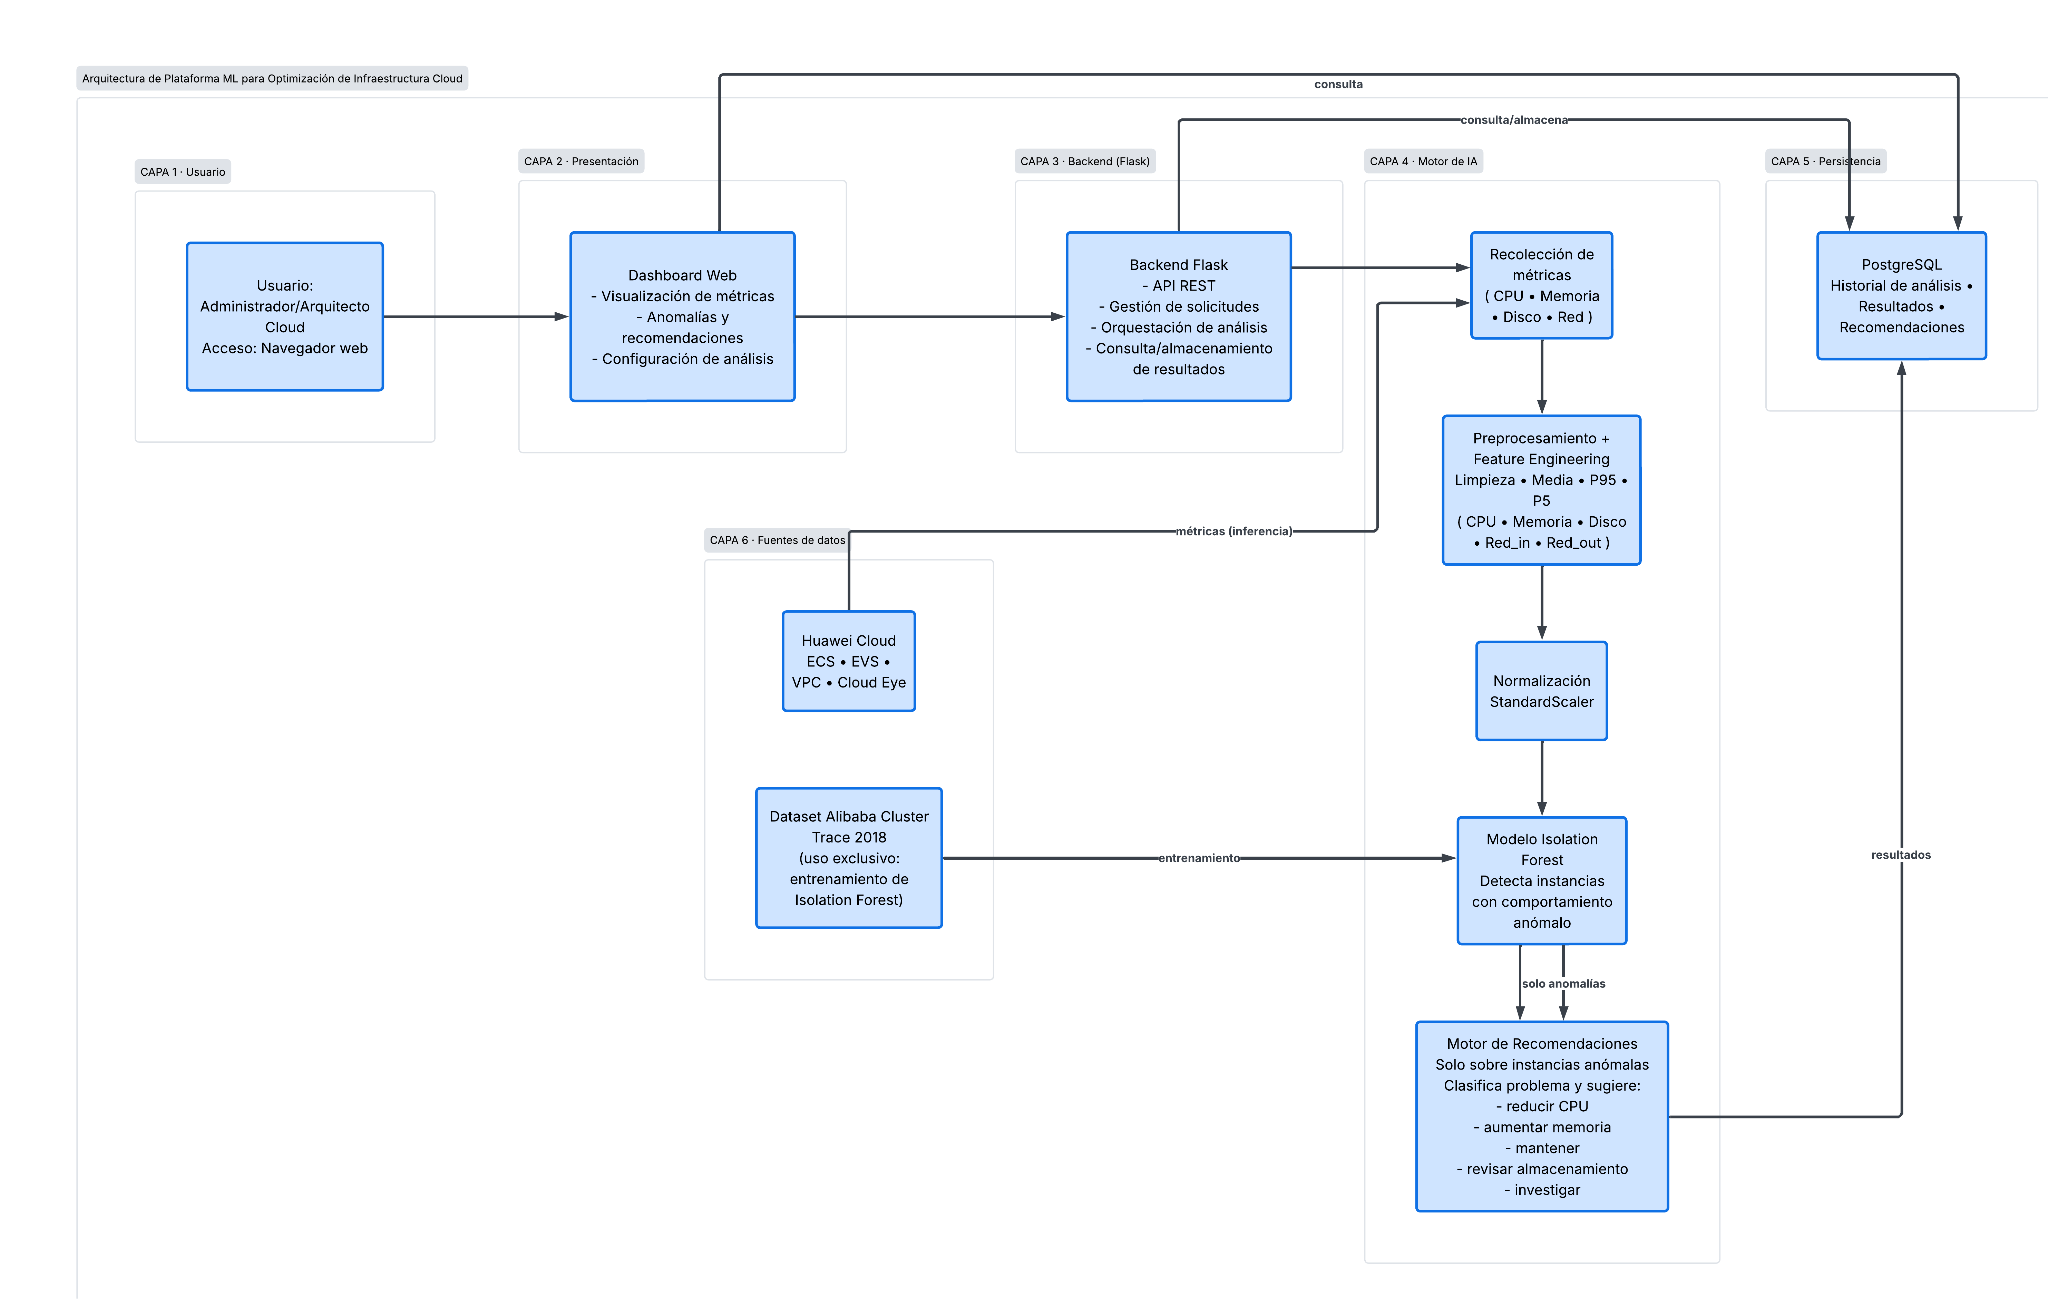
\includegraphics[width=0.9\textwidth]{media/image4.png}
\caption{Diagrama de arquitectura de la solución}
\label{fig:arquitectura}
\end{figure}

\section{Modelo Entidad-Relación}

El Diagrama Entidad-Relación presentado en la Figura representa el modelo de datos diseñado para la plataforma de optimización de infraestructuras cloud. El modelo establece una separación entre las distintas etapas de procesamiento de la plataforma. Las métricas representan el comportamiento observado de las instancias, los análisis representan las ejecuciones del modelo de detección, los resultados de anomalía representan las decisiones obtenidas mediante Isolation Forest y las recomendaciones representan las acciones de optimización derivadas de dichas detecciones. Esta estructura permite mantener la trazabilidad del proceso completo, desde los datos de utilización de los recursos hasta la generación de una recomendación de optimización.

\begin{figure}[H]
\centering
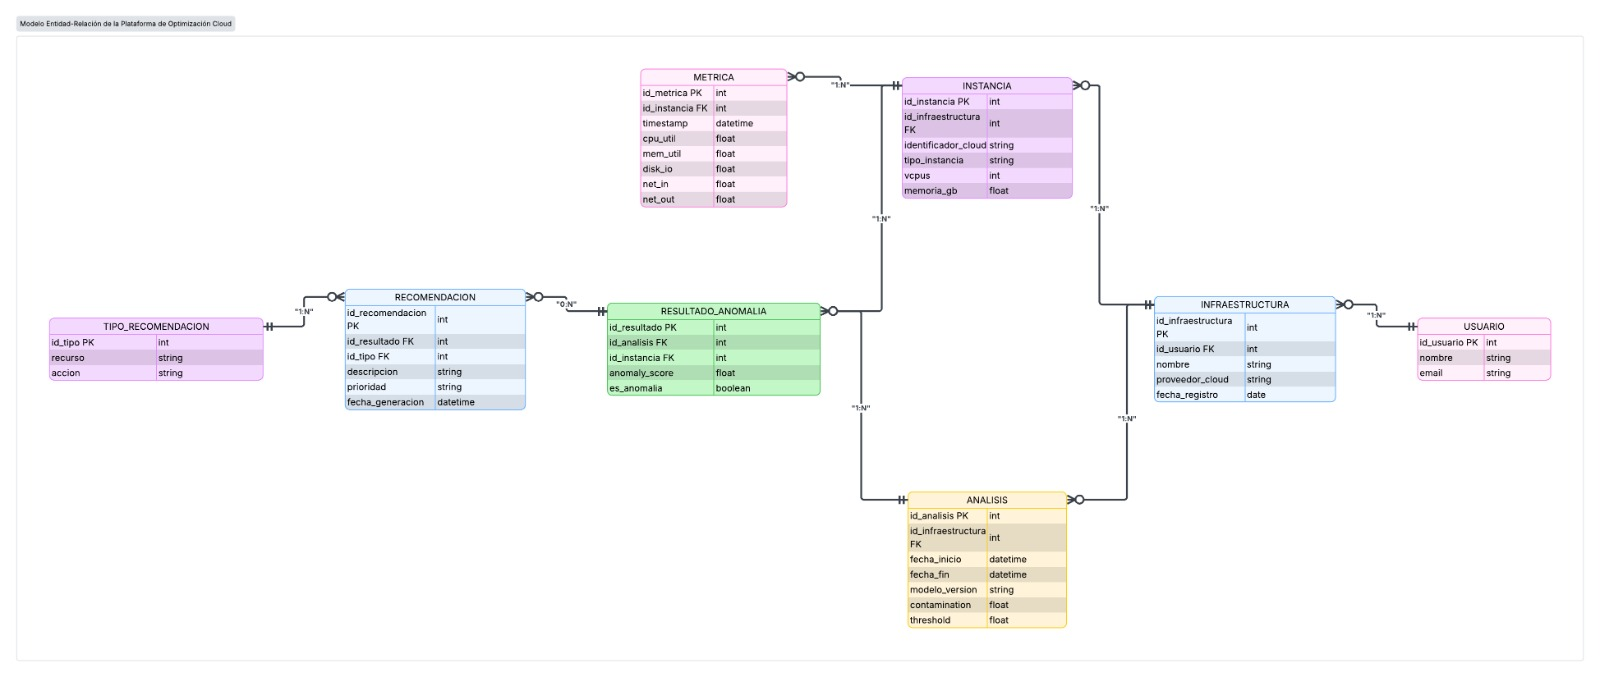
\includegraphics[width=0.9\textwidth]{media/image2.png}
\caption{Modelo Entidad-Relación de la plataforma}
\label{fig:er}
\end{figure}
